\subsection{Base radiale (RBF)}
\newcommand{\factnorm}{\sum_{r=1}^{m}x_{r}}
\subsubsection{Neurone}
Un neurone \textbf{caché} d'un \rbf n'effectue pas de somme pondérée de ses entrées. Il applique directement sa fonction
\[\phi(x) = e^{-\frac{1}{2}\sum_{k=1}^{n}\frac{(x_k-\mu_{ik})^2}{\sigma_{ik}^{2}}}\]
Une gaussienne de moyenne $\mu$ et d'écart-type $\sigma$ où $x$, de dimension $n$, est l'entrée du neurone et $i$ l'indice du neurone.
%$\phi(x)$ peut se résumer en: \[\phi(x) = e^{-\beta||x-\mu||^2}\]Où $\beta$ est donc un coefficient qui règle la largeur de la courbe en cloche.\\
\\

Un neurone \textbf{de sortie} d'un \rbf n'effectue pas non plus de somme pondérée de ses entrées. Sa fonction d'activation est:
\[\phi(x) = \frac{\sum_{j=1}^{m}W_{ij}x_{j}}{\sum_{j=1}^{m}x_{j}}\]
Où $i$ est l'indice du neurone et $x$ l'entrée de dimension $m$.
\begin{figure}
 \centering
 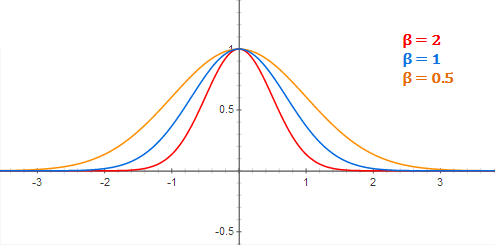
\includegraphics[scale=0.7]{../figures/RBFactivation.png}
 \caption{Activation d'un neurone RBF avec différentes valeurs d'écart-type}
 \label{rbfactivation}
\end{figure}
La Figure \ref{rbfactivation} représente la sortie d'un neurone \rbf où $\mu$ et $x$ sont de dimension 1 et $\mu = 0$.\\
Pour résumer, un neurone \rbf renvoie une valeur indiquant la simularité entre l'entrée et son prototype.
\subsubsection{Structure}
\begin{figure}
 \centering
 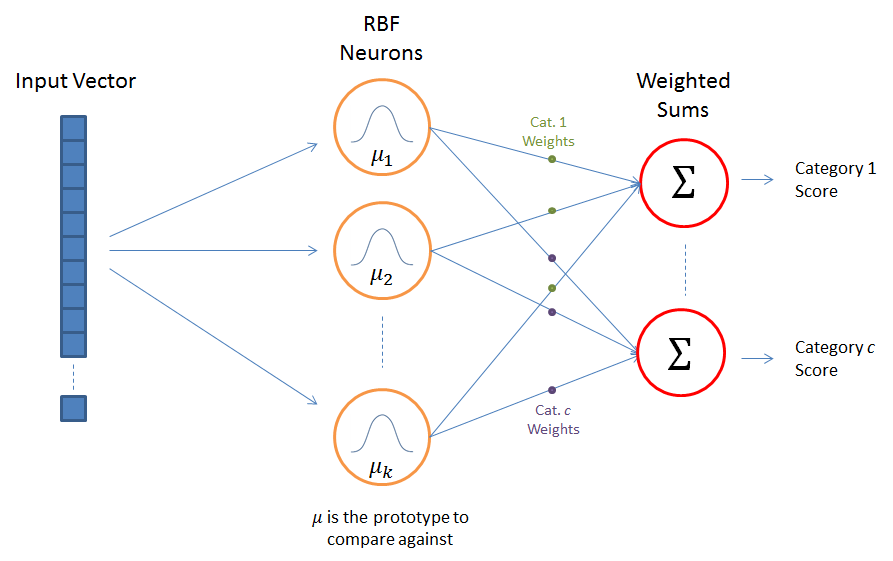
\includegraphics[scale=0.5]{../figures/RBFstruct.png}
 \caption{Structure RBF. \textbf{Source}: McCormick\cite{RBFtuto}}
 \label{structurerbf}
\end{figure}
La structure d'un \rbf est comme celle du \mlp sauf qu'il n'y a qu'une seule couche cachée (Figure \ref{structurerbf}).
\subsubsection{Apprentissage}
Dans ce réseau, les paramètres qui seront modifiés lors de l'apprentissage sont les poids des neurones de sortie et les moyennes et écart-types des neurones cachés.
Reprenons l'erreur quadratique $Q$ défini dans la section \ref{sec:appmlp}.
Les paramètres devront être modifiés de la sorte:
\[\Delta W_{ij} = -\eta \partiel{Q}{W_{ij}}, \Delta \mu_{ik} = -\eta \partiel{Q}{\mu_{ik}}, \Delta \sigma_{ik} = \eta \partiel{Q}{\sigma_{ik}}\]
On a vu dans la section \ref{sec:appmlp} que si $\phi_i$ est la sortie de la fonction d'activation d'un neurone de sortie $i$ et $s_i$ la sortie attendue du neurone $i$,
\[\partiel{Q}{\phi_i} = (\phi_i - s_i)\]
Ensuite, toujours avec $i$ un \textbf{neurone de sortie},
\begin{equation}
 \begin{split}
  \partiel{\phi_i}{W_{ij}} & = \partiel{\frac{\sum_{r=1}^{m}W_{ir}x_{j}}{\factnorm}}{W_{ij}}\\
  ~ & = \frac{1}{\factnorm} \partiel{\sum_{r=1}^{m}W_{ir}x_{j}}{W_{ij}}\\
  ~ & = \frac{1}{\factnorm} \partiel{\left(W_{i1}x_1 + W_{i2}x_2 + ... + W_{ij}x_j + ... + W_{im}x_m\right)}{W_{ij}}\\
  ~ & = \frac{1}{\factnorm} \left(\partiel{W_{i1}x_1}{W_{ij}} + \partiel{W_{i2}x_2}{W_{ij}} + ... + \partiel{W_{ij}x_j}{W_{ij}} + ... + \partiel{W_{im}x_m}{W_{ij}}\right)\\
  ~ & = \frac{1}{\factnorm} \left(0 + 0 + ... + x_j + ... + 0\right)\\
  ~ & = \frac{x_j}{\factnorm}
 \end{split}
\end{equation}\label{eq:b}
$\Delta W_{ij} = -\eta (\phi_i - s_i) \frac{x_j}{\factnorm}$\\

Maitenant, si $i$ est un \textbf{neurone caché}, $\Delta\mu_{ik} = -\eta\partiel{Q}{\mu_{ik}}$ et $\Delta\sigma_{ik} = -\eta\partiel{Q}{ik}$.
\begin{equation}
 \begin{split}
 \Delta \mu_{ik} & = -\eta \partiel{Q}{\mu_{ik}}\\
 \partiel{Q}{\mu_{ik}} & = \partiel{Q}{\phi_i} \partiel{\phi_i}{\mu_{ik}}\\
 \partiel{Q}{\phi_i} & = \sum_{j} \partiel{Q}{\phi_j}\partiel{\phi_j}{\phi_i}
 \end{split}
\end{equation}
Où $j$ est un neurone de sortie. Or
\begin{equation}
 \begin{split}
 \partiel{Q}{\phi_j} & = (\phi_j - s_j)
 \end{split}
\end{equation}
Et posons $x_r$ l'entrée de $j$ provenant de $i$. On a donc que $\phi_i = x_r$.
Posons $n$ la dimension de l'entrée de $j$.
Posons aussi $R = \sum_{k=1}{n}x_k$.
On a que
\begin{equation}
 \begin{split}
 \partiel{\frac{1}{R}}{x_k} & = \frac{-1}{R^2}\partiel{R}{x_k}\\
 ~ & = \frac{-1}{R^2}\partiel{x_1+x_2+...+x_k+...+x_n}{x_k}\\
 ~ & = \frac{-1}{R^2} 1
 \end{split}
\end{equation}
Dès lors,
\begin{equation}
 \begin{split}
 \partiel{\phi_j}{\phi_i} & = \partiel{\phi_j}{x_r}\\
 ~ & = \partiel{\left(\frac{\sum_{k=1}^{n}W_{jk}x_k}{\sum_{k=1}{n}x_k}\right)}{x_r}\\
 ~ & = \partiel{\left(\frac{W_{j1}x_1}{R} + \frac{W_{j2}x_2}{R} + ... + \frac{W_{jr}x_r}{R} + ... + \frac{W_{jn}x_n}{R}\right)}{x_r}\\
 ~ & = \partiel{\left(\frac{W_{j1}x_1}{R}\right)}{x_r} + \partiel{\left(\frac{W_{j2}x_2}{R}\right)}{x_r} + ... + \partiel{\left(\frac{W_{jr}x_r}{R}\right)}{x_r} + .. + \partiel{\left(\frac{W_{jn}x_n}{R}\right)}{x_r}\\
 ~ & = (W_{j1}x_1)\frac{-1}{R^2} + (W_{j2}x_2)\frac{-1}{R^2} + ... + \left[(W_{jr}x_r)\partiel{\frac{1}{R}}{x_r}+\partiel{(W_{jr}x_r)}{x_r}\frac{1}{R}\right] + ... + (W_{jn}x_n)\frac{-1}{R^2}\\
 ~ & = (W_{j1}x_1)\frac{-1}{R^2} + (W_{j2}x_2)\frac{-1}{R^2} + ... + \left[(W_{jr}x_r)\frac{-1}{R^2}+W_{jr}\frac{1}{R}\right] + ... + (W_{jn}x_n)\frac{-1}{R^2}\\
 ~ & = \left(\sum_{k=1}^{n}W_{jk}x_k\frac{-1}{R^2}\right)-W_{jr}x_r\frac{-1}{R^2} + \left[(W_{jr}x_r)\frac{-1}{R^2}+W_{jr}\frac{1}{R}\right]\\
 ~ & = \frac{-1}{R^2} \left[\left(\sum_{k=1}^{n}W_{jk}x_k\right)-W_{jr}x_r + (W_{jr}x_r) + W_{jr}(-R)\right]\\
 ~ & = \frac{-1}{R^2} \left(W_{jr}(-R) + \sum_{k=1}^{n}W_{jk}x_k\right)\\
 ~ & = \frac{1}{R^2} \left(W_{jr}R - \sum_{k=1}^{n}W_{jk}x_k\right)
 \end{split}
\end{equation}
Ensuite,
\[\partiel{\phi_i}{\mu_{ik}} = \phi_i \frac{x_k-\mu_{ik}}{\sigma_{ik}^2}\]
Au final,
\[\Delta\mu_{ik} = -\eta \left[\sum_{i}(\phi_j - s_j) \frac{1}{R^2} \left(W_{jr}R - \sum_{k=1}^{n}W_{jk}x_k\right)\right] \phi_i\frac{x_k-\mu_{ik}}{\sigma_{ik}^2}\]
si $i$ est un \textbf{neurone caché},
\begin{equation}
 \begin{split}
 \Delta \sigma_{ik} & = -\eta \partiel{Q}{\sigma_{ik}}\\
 ~ & = -\eta \partiel{Q}{\phi_j} \partiel{\phi_j}{\phi_i} \partiel{\phi_i}{\sigma_{ik}}
 \end{split}
\end{equation}
Or \[\partiel{\phi}{\sigma_{ik}} = \phi_i \frac{(x_k-\mu_{ik})^2}{\sigma_{ik}^3}\]
Au final,
\[\Delta \sigma_{ik} = -\eta \left[\sum_{i}(\phi_j - s_j) \frac{1}{R^2} \left(W_{jr}R - \sum_{k=1}^{n}W_{jk}x_k\right)\right] \phi_i \frac{(x_k-\mu_{ik})^2}{\sigma_{ik}^3}\]
\subsubsection{Applications}
Un \rbf peut aussi servir pour la classification non linéaire.\cite{statistica}